%%% Document Formatting
\documentclass[12pt,fleqn]{article}
\usepackage[a4paper,
            bindingoffset=0.2in,
            left=0.75in,
            right=0.75in,
            top=0.8in,
            bottom=0.8in,
            footskip=.25in]{geometry}
\setlength\parindent{10pt}

%%% Imports
\usepackage{amsmath}
\numberwithin{equation}{section}
\usepackage{amsfonts}
\usepackage{amssymb}
\usepackage{mathtools}
\usepackage{cancel}
\usepackage{empheq}
\usepackage[ruled,lined,linesnumbered]{algorithm2e}

\newtheorem{theorem}{Theorem}
\newtheorem{definition}{Definition}
\newtheorem{proposition}{Proposition}
\newtheorem{lemma}{Lemma}
\newtheorem{example}{Example}
\newtheorem{fact}{Fact}
\newtheorem{corollary}{Corollary}
\newtheorem{remark}{Remark}

\newcommand{\expect}[1]{\mathbb{E}\left[#1\right]}
\newcommand{\KL}[2]{D_{\mathrm{KL}}\!\left(#1 \,\|\, #2\right)}
\newcommand{\R}{\mathbb{R}}
\newcommand{\N}{\mathcal{N}}
\newcommand{\I}{\mathbb{I}}
\newcommand{\X}{\mathcal{X}}
\newcommand{\Y}{\mathcal{Y}}
\newcommand{\Law}{\mathrm{Law}}

% Visualization
\usepackage{graphicx}
\usepackage{tikz}

%%% Formatting
\usepackage{hyperref}
\hypersetup{
    colorlinks=true,
    linkcolor=blue,
    filecolor=magenta,      
    urlcolor=cyan,
    pdftitle={SCSI Lecture Notes},
    pdfpagemode=FullScreen,
}
\urlstyle{same}

\usepackage{mdframed}
\newmdenv[ 
  topline=false,
  bottomline=false,
  skipabove=\topsep,
  skipbelow=\topsep
]{sidework}

\newmdenv[
  linecolor=blue!50,
  backgroundcolor=blue!5,
  linewidth=1pt,
  roundcorner=5pt,
  skipabove=\topsep,
  skipbelow=\topsep
]{keybox}

%%%%% ------------------ %%%%%
\title{Self-Consistent Stochastic Interpolants \\ 
\large Lecture Notes on Modi, Han, Vanden-Eijnden \& Bruna (2025)}
\author{Clark Miyamoto (cm6627@nyu.edu)}
\date{\today}
\begin{document}

\maketitle

\tableofcontents
\newpage

%% ============================================================
\section{Problem Setup: Inverse Problems from Corrupted Data}
%% ============================================================

\subsection{Setting}
You are given:
\begin{itemize}
	\item A dataset $\{y_i\}_i$ of experimental measurements $y_i \in \Y$, each arising from an underlying signal $x_i \in \X$.
	\item Oracle access to a forward model $\mathcal F(x) = y$ which you believe accurately represents the data (no model misspecification). The forward model can be stochastic, hence non-invertible at the level of individual samples. It implicitly defines a conditional distribution $P(dy \mid x)$.
\end{itemize}
We write $\Law(y) = \mu$ for the observation distribution, and define the integral operator $\mathcal K : \mathcal P(\X) \to \mathcal P(\Y)$ via
\[
	(\mathcal K \pi)(A) = \int_\X P(A \mid x) \, \pi(dx).
\]
The key relationship is:
\begin{equation}
	\mathcal K \pi = \mu. \label{eq:forward}
\end{equation}

\noindent\textbf{Goal.} Given a new observation $y$, recover the signal $x$. This is an \textbf{inverse problem}. Note this differs from Bayesian inference: we are not assuming an explicit prior on $x$, but rather trying to recover the prior $\pi$ itself from the data.

\begin{sidework}
\noindent\textbf{Examples:}
\begin{itemize}
	\item \textbf{Reconstruction:} $y$ is a CT scan, $x$ is the 3D tissue model, $\mathcal F$ is the Radon transform.
	\item \textbf{Camera Sensor + Lens:} $y$ is an observed spectrum, $x$ is the true spectrum, $\mathcal F$ models atmospheric distortion, finite resolution, and detector noise.
\end{itemize}
\end{sidework}

\subsection{Injectivity at the Distribution Level}
Although $\mathcal F$ is typically ill-conditioned or non-invertible as a map on individual samples, the situation improves at the level of distributions. If $\mathcal K$ is \textbf{injective}---meaning $\mathcal K \pi = \mathcal K \tilde\pi$ implies $\pi = \tilde\pi$---then we can hope to recover $\pi$ from $\mu$.

\begin{example}[AWGN Channel]
If $\mathcal F(x) = x + \sigma \xi$ with $\xi \sim \N(0, \I)$, then $\mu = \pi \star \gamma_\sigma$ (convolution with a Gaussian). By the injectivity of the characteristic function under convolution, $\mathcal K$ is injective for any $\sigma < \infty$.
\end{example}

%% ============================================================
\section{The Self-Consistency Idea}
%% ============================================================

\subsection{High-Level Argument}

Consider a generative model $\Phi_\Theta$ (the full backward ODE/SDE integration) that maps observations to reconstructed signals. If $y \sim \mu$, then $\Phi_\Theta(y) = x$ implicitly defines a pushforward:
\begin{equation}
	(\Phi_\Theta)_\# \mu = \pi_\Theta. \label{eq:gen_push}
\end{equation}

Suppose we have somehow trained $\Phi_\Theta$ so that $\pi_\Theta \approx \pi$. Applying the forward model to the generated samples and using \eqref{eq:forward}:
\begin{equation}
	\mathcal K \pi_\Theta = \mathcal K (\Phi_\Theta)_\# \mu \approx \mathcal K \pi = \mu.
\end{equation}

At a fixed point, this becomes the 
\begin{keybox}
\textbf{Self-consistency equation}
\begin{equation}
	\mathcal K (\Phi_{\Theta^*})_\# \mu = \mu. \label{eq:selfconsist}
\end{equation}
\end{keybox}

\noindent\textbf{Interpretation:} The properly trained generative model $\Phi_{\Theta^*}$ maps noisy observations $\mu$ to clean signals $\pi_{\Theta^*}$. Passing these through the forward model $\mathcal K$ should recover $\mu$. The generative model is an ``inverse'' of $\mathcal K$ at the distribution level.

\subsection{Review of Stochastic Interpolants}

A stochastic interpolant between distributions $\pi$ (data) and $\mu$ (observations) is
\begin{equation}
	I_t = \alpha_t \, x_0 + \beta_t \, x_1 + \gamma_t \, z, \qquad t \in [0,1], \label{eq:SI}
\end{equation}
where $(x_0, x_1) \sim \nu(dx_0, dx_1)$ is drawn from a coupling with marginals $\int \nu(\cdot, dx_1) = \pi$ and $\int \nu(dx_0, \cdot) = \mu$, the noise $z \sim \N(0, \I)$ is independent, and the schedules satisfy boundary conditions $\alpha_0 = \beta_1 = 1$, $\alpha_1 = \beta_0 = 0$, $\gamma_0 = \gamma_1 = 0$.

The velocity field and denoiser are defined as conditional expectations:
\[
	b(t,x) := \mathbb E[\dot I_t \mid I_t = x], \qquad g(t,x) := \mathbb E[z \mid I_t = x].
\]
These are learned via least-squares regression:
\begin{align}
	\mathcal L_b(\hat b) &= \int_0^1 \mathbb E\bigl[|\hat b_t(I_t) - \dot I_t|^2\bigr]\, dt, \label{eq:driftloss} \\
	\mathcal L_g(\hat g) &= \int_0^1 \mathbb E\bigl[|\hat g_t(I_t) - z|^2\bigr] \, dt. \label{eq:denoiserloss}
\end{align}

At inference, one integrates the reverse-time SDE:
\begin{equation}
	dX_t^B = \bigl[\hat b_t(X_t^B) + \epsilon_t \gamma_t^{-1} \hat g_t(X_t^B)\bigr] dt + \sqrt{2\epsilon_t}\, dW_t^B, \label{eq:reverseSDE}
\end{equation}
where $\epsilon_t \geq 0$ is the diffusion coefficient. Setting $\epsilon_t = 0$ recovers the probability flow ODE.

\subsection{Enforcing Self-Consistency via Iteration}

In the standard setting, one needs paired samples from $\pi$ and $\mu$ to train the interpolant. In our setup, we only have access to $y \sim \mu$ and the forward model $\mathcal F$. If we had samples $x \sim \pi$, we could build the interpolant
\begin{equation}
	I_t = \alpha_t \, x + \beta_t \, \mathcal F(x) + \gamma_t \, z, \label{eq:oracle_interp}
\end{equation}
since $\mathcal F(x) \sim \mu$. This has correct boundary conditions: $I_0 \sim \pi$ and $I_1 \sim \mu$.

Since we lack samples from $\pi$, we use the current model's output as a proxy:
\begin{keybox}
\textbf{Self-Consistent Stochastic Interpolant}
\begin{equation}
	I_t^{(k+1)} = \alpha_t \, \Phi_{\Theta^{(k)}}(y) + \beta_t \, \mathcal F\bigl(\Phi_{\Theta^{(k)}}(y)\bigr) + \gamma_t \, z, \qquad y \sim \mu,\; z \sim \N(0,\I). \label{eq:scsi}
\end{equation}
This leads to a bi-level iterative scheme:
\begin{equation}
	\Theta^{(k)} \xrightarrow[\text{`E' step}]{\text{via \eqref{eq:scsi}}} I^{(k+1)}_t \xrightarrow[\text{`M' step}]{\text{minimize \eqref{eq:driftloss}\eqref{eq:denoiserloss} with } I^{(k+1)}_t} \Theta^{(k+1)}.
\end{equation}
\end{keybox}
To be precise, here's the pseudocode for SCSI.\\

\begin{algorithm}[H]
\caption{Training of Self-Consistent Stochastic Interpolant (SCSI)}
\KwIn{Observation distribution $\mu$, forward model $\mathcal{F}$, schedule $(\alpha_t, \beta_t, \gamma_t)$, initial parameters $\Theta^{(0)}$, outer iterations $K$, inner steps $T_{\text{tr}}$}
\KwOut{Optimized parameters $\Theta^{(K)}$}
$\Theta \leftarrow \Theta^{(0)}$\;
\For{$k = 1, \ldots, K$}{
    \For{$i = 1, \ldots, T_{\text{tr}}$}{
        Sample $y \sim \mu$\;
        $x = \Phi_{\Theta^{(k-1)}}(y)$ \tcp*{backward transport}
        $\tilde{y} = \mathcal{F}(x)$ \tcp*{forward model}
        Sample $z \sim \mathcal{N}(0, \I)$,\; $t \sim \mathcal{U}(0, 1)$\;
        $I_t = \alpha_t \, x + \beta_t \, \tilde{y} + \gamma_t \, z$\;
        SGD update of $\Theta$ via losses \eqref{eq:driftloss}--\eqref{eq:denoiserloss}\;
    }
    $\Theta^{(k)} \leftarrow \Theta$\;
}
\Return{$\Theta^{(K)}$}
\end{algorithm}
In practice, the inner loop need not converge: setting $T_\text{tr} = 1$ (with stop-gradient on $I_t$) already works well empirically.


%% ============================================================
\section{Case Study: AWGN Channel with Gaussian Prior} \label{sec:gaussian}
%% ============================================================

We now specialize to a toy problem where everything stays Gaussian, allowing closed-form analysis. This serves two purposes: (i) verify convergence and compute its rate, and (ii) compare SCSI against the EM algorithm.

\subsection{Setup}

\begin{itemize}
    \item \textbf{True data distribution (unknown):} $\pi = \N(b, \Sigma)$ with $\Sigma \succ 0$.
    \item \textbf{Forward model:} $\mathcal F(x) = x + w$ where $w \sim \N(0, \I)$, independently of $x$. The observation distribution is $\mu = \N(b, \Sigma + \I)$.
    \item \textbf{Interpolant:} We use 
    \begin{equation}
        I_t = (1-\sqrt{t})\,x + \sqrt{t}\,\mathcal F(x) = x + \sqrt{t}\,w, \label{eq:gaussinterp}
    \end{equation}
    with schedule $\alpha_t = 1-\sqrt{t}$, $\beta_t = \sqrt{t}$, $\gamma_t = 0$.
    \item \textbf{Initial guess:} $\pi^{(0)} = \N(b_0, \Sigma_0)$ with $\Sigma_0 \succ 0$.
\end{itemize}

\begin{sidework}
\noindent\textbf{Why this interpolant?} With $\alpha_t = 1-\sqrt{t}$ and $\beta_t = \sqrt{t}$, if $x \sim \N(\tilde b, \tilde \Sigma)$ and $w \sim \N(0,\I)$ independently, then
\[
	I_t = x + \sqrt{t}\, w \sim \N(\tilde b, \tilde\Sigma + t\,\I).
\]
This is exactly the heat semigroup: $\Law(I_t) = e^{\frac{t}{2}\Delta} \N(\tilde b, \tilde\Sigma)$. The forward process satisfies
\[
	\partial_t p_t = \tfrac{1}{2} \Delta p_t, \qquad p_0 = \N(\tilde b, \tilde\Sigma),
\]
so the law of the interpolant evolves under the heat equation. This is what makes the entire Gaussian calculation tractable---the reverse process becomes an Ornstein--Uhlenbeck process with an explicit solution.
\end{sidework}

\noindent Because of the Gaussian structure, every iterate stays Gaussian: $\pi^{(k)} = \N(b_k, \Sigma_k)$.

\subsection{Roadmap}
\begin{enumerate}
    \item Solve the reverse SDE to find the update rule: given $\pi^{(k)}$, what is $\pi^{(k+1)}$?
    \item Extract the contraction rate and determine convergence.
    \item Compare with the EM algorithm.
\end{enumerate}

\subsection{Step 1: The Reverse Process and Update Rule}

\subsubsection{Forward process}

Fix the current iterate $\pi^{(k)} = \N(b_k, \Sigma_k)$. The law of $I_t$ is
\begin{equation}
	p_t = \N(b_k, \Sigma_k + t\,\I), \label{eq:pt}
\end{equation}
evolving under $\partial_t p_t = \frac{1}{2}\Delta p_t$ with terminal condition $p_1 = \N(b_k, \Sigma_k + \I) = \mathcal K \pi^{(k)}$.

\subsubsection{Reverse SDE}

We reverse time via $\tau = 1 - t$ and set $q_\tau := p_{1-\tau}$. Then $\partial_\tau q_\tau = -\frac{1}{2}\Delta q_\tau$. Introducing a diffusion coefficient $\epsilon \geq 0$ by splitting the Laplacian:
\begin{equation}
	\partial_\tau q_\tau = -\nabla \cdot \!\left[\frac{1+\epsilon}{2}(\nabla \log q_\tau)\, q_\tau\right] + \frac{\epsilon}{2}\Delta q_\tau. \label{eq:reverseFP}
\end{equation}
This is the Fokker--Planck equation for the reverse SDE:
\begin{equation}
	dY_\tau = \frac{1+\epsilon}{2}\nabla\log q_\tau(Y_\tau)\,d\tau + \sqrt{\epsilon}\,dW_\tau. \label{eq:revSDE}
\end{equation}

\subsubsection{Score for Gaussians}

From \eqref{eq:pt}, the score of $p_t$ is
\[
	\nabla \log p_t(x) = -(\Sigma_k + t\,\I)^{-1}(x - b_k).
\]
Substituting $q_\tau = p_{1-\tau}$:
\begin{equation}
	\nabla \log q_\tau(x) = -\bigl(\Sigma_k + (1-\tau)\I\bigr)^{-1}(x - b_k). \label{eq:score}
\end{equation}

Plugging into \eqref{eq:revSDE}:
\begin{equation}
	dY_\tau = -\frac{1+\epsilon}{2}\bigl(\Sigma_k + (1-\tau)\I\bigr)^{-1}(Y_\tau - b_k)\,d\tau + \sqrt{\epsilon}\,dW_\tau. \label{eq:revSDE_explicit}
\end{equation}

\subsubsection{Solving the reverse SDE}

This is a linear SDE (Ornstein--Uhlenbeck process). We center by $\tilde Y_\tau = Y_\tau - b_k$:
\[
	d\tilde Y_\tau = A(\tau)\,\tilde Y_\tau\,d\tau + \sqrt{\epsilon}\,dW_\tau, \qquad A(\tau) := -\frac{1+\epsilon}{2}(\Sigma_k + (1-\tau)\I)^{-1}.
\]

\begin{sidework}
\noindent\textbf{Fundamental solution.} We seek a matrix $\Phi(\tau,s)$ satisfying
\[
	\frac{\partial}{\partial\tau}\Phi(\tau,s) = A(\tau)\Phi(\tau,s), \qquad \Phi(s,s) = \I.
\]
Since $\Sigma_k$ is symmetric, $A(\tau)$ and $A(\tau')$ share a common eigenbasis for all $\tau, \tau'$ (they are all functions of $\Sigma_k$). Therefore the matrix exponential simplifies:
\[
	\Phi(\tau,s) = \exp\!\left(\int_s^\tau A(u)\,du\right).
\]
Evaluating component-wise on each eigenvalue $\lambda_i$ of $\Sigma_k$ (via the substitution $v = 1-u$):
\[
	\int_s^\tau \frac{du}{\lambda_i + 1 - u} = \log\frac{\lambda_i + 1 - s}{\lambda_i + 1 - \tau}.
\]
Therefore:
\begin{equation}
	\Phi(\tau,s) = \left[(\Sigma_k + (1-\tau)\I)(\Sigma_k + (1-s)\I)^{-1}\right]^{(1+\epsilon)/2}. \label{eq:fundsoln}
\end{equation}
\end{sidework}

Integrating the SDE with the variation-of-constants formula:
\begin{equation}
	Y_\tau = b_k + \Phi(\tau,0)(Y_0 - b_k) + \sqrt{\epsilon}\int_0^\tau \Phi(\tau,s)\,dW_s. \label{eq:Ysoln}
\end{equation}

\subsubsection{Evaluating at $\tau = 1$ to get $\pi^{(k+1)}$}

At $\tau = 1$, the reverse SDE has mapped $Y_0 \sim \mu = \N(b, \Sigma + \I)$ (the \emph{true} observation distribution, which provides our input data) through the flow defined by the \emph{current} model's score. This gives us $Y_1 \sim \pi^{(k+1)}$.

From \eqref{eq:fundsoln}, the key matrix is:
\begin{equation}
	\Phi(1,0) = \bigl[\Sigma_k(\Sigma_k + \I)^{-1}\bigr]^{(1+\epsilon)/2} =: B_k. \label{eq:Bk}
\end{equation}

\textbf{Mean of $Y_1$:} Since $\mathbb E[Y_0] = b$ (the true mean, since $Y_0 \sim \mu$):
\[
	\mathbb E[Y_1] = b_k + B_k(b - b_k).
\]

\textbf{Covariance of $Y_1$:} Two independent contributions:
\begin{enumerate}
	\item \emph{Deterministic part:} $\Phi(1,0)(Y_0 - b_k)$ has covariance $B_k(\Sigma + \I)B_k$ (since $\mathrm{Cov}(Y_0) = \Sigma + \I$).
	\item \emph{Stochastic integral:} $\sqrt{\epsilon}\int_0^1 \Phi(1,s)\,dW_s$ has covariance
	\[
		\epsilon \int_0^1 \Phi(1,s)\Phi(1,s)^\top ds.
	\]
	Using \eqref{eq:fundsoln} and evaluating the integral on the eigenbasis of $\Sigma_k$, the $i$-th eigenvalue contributes
	\[
		\epsilon \int_0^1 \left(\frac{\lambda_i}{\lambda_i + 1-s}\right)^{1+\epsilon} ds = \lambda_i^{1+\epsilon}\cdot\frac{(\lambda_i+1)^\epsilon - \lambda_i^\epsilon}{\epsilon}.
	\]
\end{enumerate}

After simplification (expanding and collecting terms), the total covariance of $Y_1$ yields:
\begin{keybox}
\textbf{Update rule:}
\begin{align}
	b_{k+1} &= b_k + B_k(b - b_k), \label{eq:mean_update}\\
	\Sigma_{k+1} &= \Sigma_k + B_k(\Sigma - \Sigma_k)B_k, \label{eq:cov_update}
\end{align}
where
\begin{equation}
	B_k = \bigl[\Sigma_k(\Sigma_k + \I)^{-1}\bigr]^{(1+\epsilon)/2}. \label{eq:Bk_def}
\end{equation}
\end{keybox}

\begin{remark}
One can verify the covariance update \eqref{eq:cov_update} directly by expanding:
\[
	\mathrm{Cov}(Y_1) = B_k(\Sigma + \I)B_k + (\text{stochastic integral covariance}) - (\text{centering}).
\]
Using $B_k(\Sigma + \I)B_k = B_k \Sigma B_k + B_k^2$ and the identity $\Sigma_k - B_k^2 \Sigma_k = \Sigma_k(I - B_k^2)$ (which follows since $B_k$ and $\Sigma_k$ commute), together with the stochastic integral term, everything collapses to $\Sigma_k + B_k(\Sigma - \Sigma_k)B_k$.
\end{remark}

\subsection{Step 2: Convergence Analysis}

We first need a simple matrix inequality.

\begin{lemma}\label{lem:matrix}
For any symmetric matrix $X$ and symmetric matrix $B$ with $0 \prec B \prec \I$:
\[
	\|X - BXB\| \leq (1 - \lambda_{\min}(B)^2)\|X\|,
\]
where $\|\cdot\| = \lambda_{\max}(\cdot)$ is the spectral norm.
\end{lemma}

We also need that the minimum eigenvalue is preserved across iterations:

\begin{lemma}[Eigenvalue preservation]\label{lem:eigenvalue}
If $\lambda_{\min}(\Sigma_0) \geq \eta$ and $\lambda_{\min}(\Sigma) \geq \eta$ for some $\eta > 0$, then $\lambda_{\min}(\Sigma_k) \geq \eta$ for all $k$.
\end{lemma}

Now we can state the main convergence result.

\begin{proposition}[Gaussian AWGN Convergence]\label{prop:convergence}
Let $\eta = \min(\lambda_{\min}(\Sigma_0), \lambda_{\min}(\Sigma))$ and assume $\eta > 0$. Then:
\begin{align}
	\|\Sigma_k - \Sigma\| &\leq \left(1 - \left(\frac{\eta}{\eta + 1}\right)^{1+\epsilon}\right)^k \|\Sigma_0 - \Sigma\|, \label{eq:cov_converge}\\
	\|b_k - b\|^2 &\leq \left(1 - \left(\frac{\eta}{\eta + 1}\right)^{1+\epsilon}\right)^k \|b_0 - b\|^2. \label{eq:mean_converge}
\end{align}
\end{proposition}

\noindent\textit{Proof of \eqref{eq:cov_converge}.} Define $R_k = \Sigma - \Sigma_k$. From \eqref{eq:cov_update}: $R_{k+1} = R_k - B_k R_k B_k$. Applying Lemma~\ref{lem:matrix}:
\[
	\|R_{k+1}\| \leq (1 - \lambda_{\min}(B_k)^2)\|R_k\|.
\]
From Lemma~\ref{lem:eigenvalue}, $\lambda_{\min}(\Sigma_k) \geq \eta$, so:
\[
	\lambda_{\min}(B_k) = \left(\frac{\lambda_{\min}(\Sigma_k)}{1 + \lambda_{\min}(\Sigma_k)}\right)^{(1+\epsilon)/2} \geq \left(\frac{\eta}{1+\eta}\right)^{(1+\epsilon)/2}.
\]
Squaring: $\lambda_{\min}(B_k)^2 \geq \left(\frac{\eta}{1+\eta}\right)^{1+\epsilon}$. Substituting and iterating gives \eqref{eq:cov_converge}. The mean convergence \eqref{eq:mean_converge} follows similarly since $b_{k+1} - b = (I - B_k)(b_k - b)$ and $\|I - B_k\| \leq 1 - \lambda_{\min}(B_k)$. \hfill$\square$

\begin{remark}[Optimal $\epsilon$]
The contraction factor $1 - \left(\frac{\eta}{\eta+1}\right)^{1+\epsilon}$ is minimized when $\epsilon = 0$ (the ODE setting). This means the probability flow ODE converges faster than any SDE formulation with $\epsilon > 0$. In the low-SNR regime $\eta \ll 1$:
\begin{itemize}
	\item ODE ($\epsilon = 0$): rate $\approx (1 - \eta)^k$,
	\item SDE with $\epsilon = 1$: rate $\approx (1 - \eta^2)^k$, which is much slower.
\end{itemize}
\end{remark}
\begin{figure*}[h!]
	\centering
	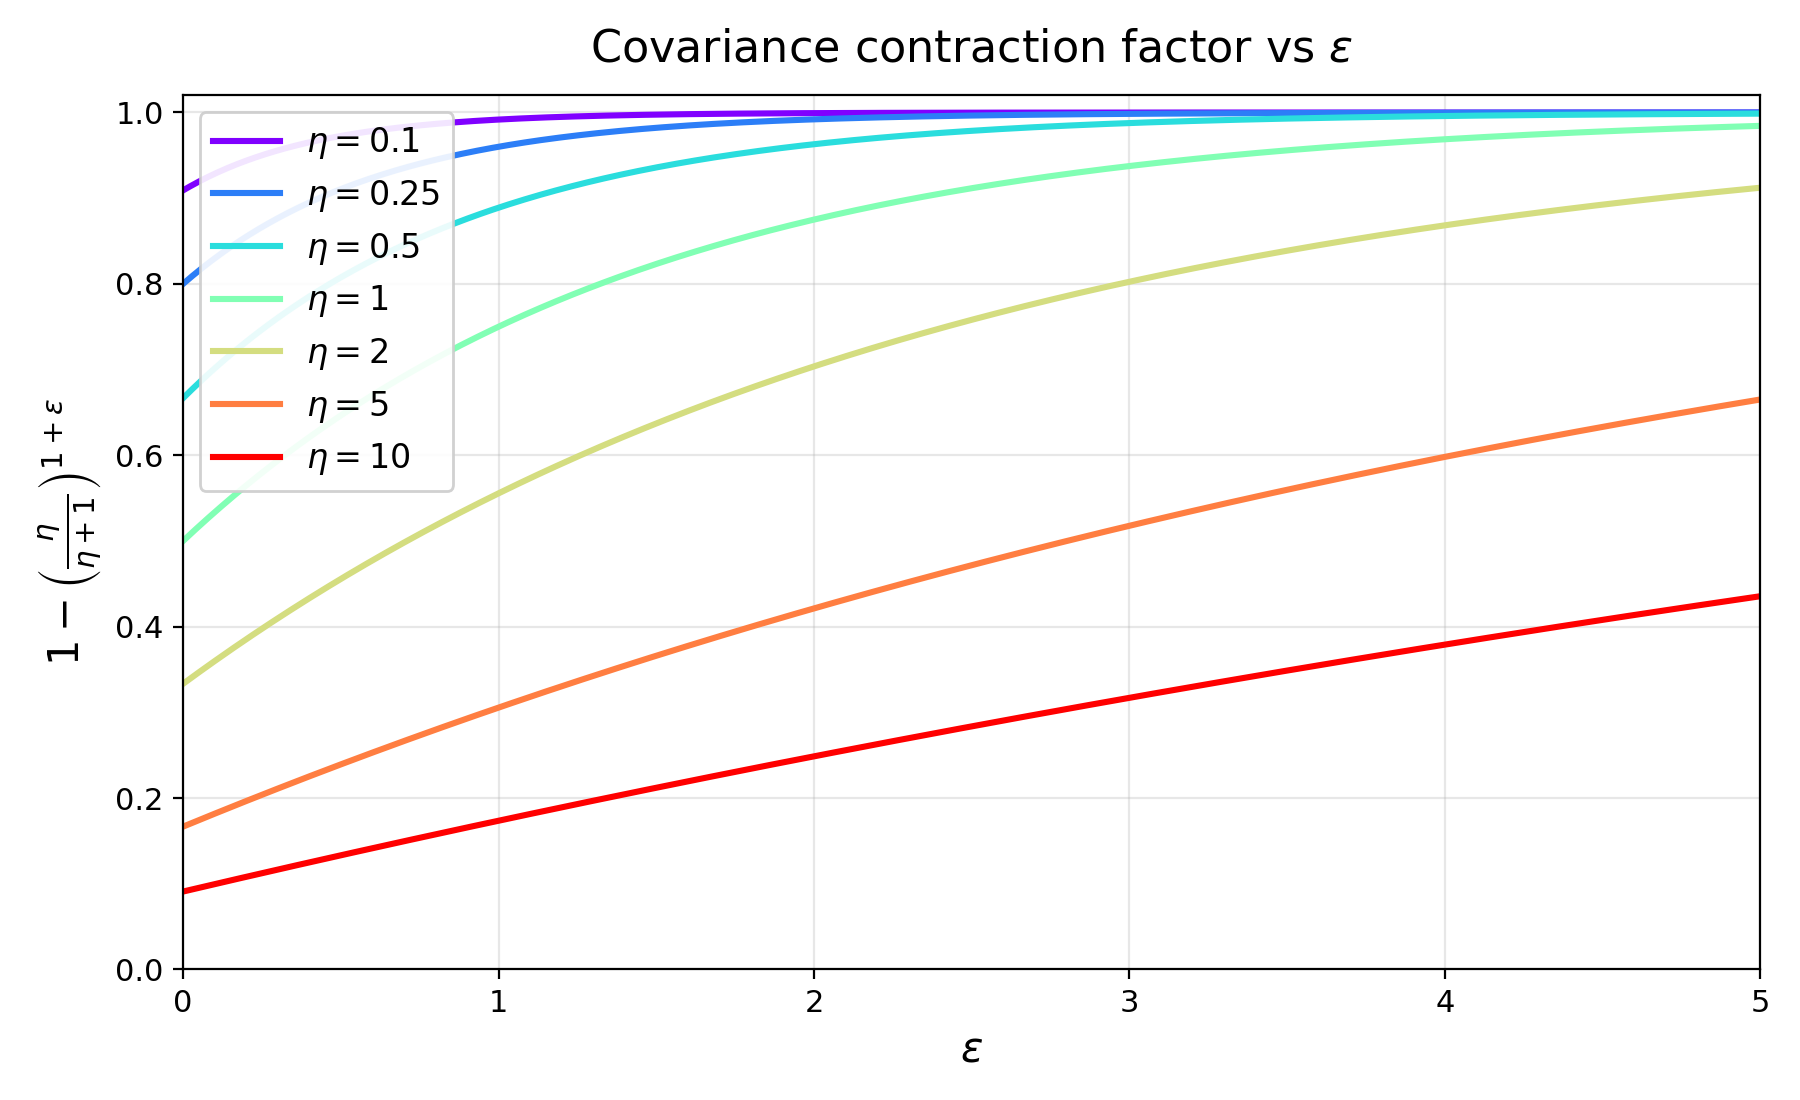
\includegraphics[scale=0.5]{contraction_rate.png}
	\caption{Contraction factor vs SDE noise level. For all SNRs $\eta$, the optimum corresponds to $\epsilon = 0$ which is using an ODE for the reverse dynamics.}
\end{figure*}

\subsection{Step 3: Comparison with the EM Algorithm} \label{sec:em}

Since we have been drawing analogies to EM, let us derive the actual EM update and compare.

\subsubsection{Deriving the EM update}

For simplicity, consider centered distributions ($b = 0$). Given the current prior $\tilde\pi_k = \N(0, \tilde\Sigma_k)$, the EM algorithm:
\\

\noindent
\textbf{E-step:} Compute the posterior $p_k(x \mid y) \propto \N(x; 0, \tilde\Sigma_k)\N(y; x, \I)$, which is Gaussian.

\noindent
\textbf{M-step:} Update the prior via the mixture
\begin{equation}
	d\tilde\pi_{k+1}(x) = \mathbb E_{y \sim \mu}\bigl[p_k(dx \mid y)\bigr]. \label{eq:EM_Mstep}
\end{equation}
Computing the Gaussian integral in \eqref{eq:EM_Mstep} explicitly yields $\tilde\pi_{k+1} = \N(0, \tilde\Sigma_{k+1})$ with:
\begin{equation}
	\tilde\Sigma_{k+1} = \tilde\Sigma_k + M_k(\Sigma - \tilde\Sigma_k)M_k, \qquad M_k = \tilde\Sigma_k(\tilde\Sigma_k + \I)^{-1}. \label{eq:EM_update}
\end{equation}

\subsubsection{EM is a special case of SCSI}

Comparing \eqref{eq:EM_update} with the SCSI update \eqref{eq:cov_update}--\eqref{eq:Bk_def}:
\[
	B_k = [\Sigma_k(\Sigma_k + \I)^{-1}]^{(1+\epsilon)/2}, \qquad M_k = \tilde\Sigma_k(\tilde\Sigma_k + \I)^{-1}.
\]
The EM update corresponds exactly to $B_k$ with exponent $(1+\epsilon)/2 = 1$, i.e., $\epsilon = 1$.

\begin{keybox}
EM corresponds to $\epsilon = 1$ in the SCSI family, which is \emph{suboptimal}. The ODE setting $\epsilon = 0$ achieves a strictly faster contraction rate. In the low-SNR regime:
\begin{center}
\begin{tabular}{lcc}
\textbf{Method}  & \textbf{Contraction rate} & \textbf{Non-asymptotic} \\
\hline
SCSI with $\epsilon = 0$ (ODE) & $(1-\eta)^k$ & $O(1/k^2)$ \\
SCSI with $\epsilon = 1$ (= EM) & $(1-\eta^2)^k$ & $O(1/k)$ \\
\end{tabular}
\end{center}
\end{keybox}

\begin{figure*}[h!]
	\centering
	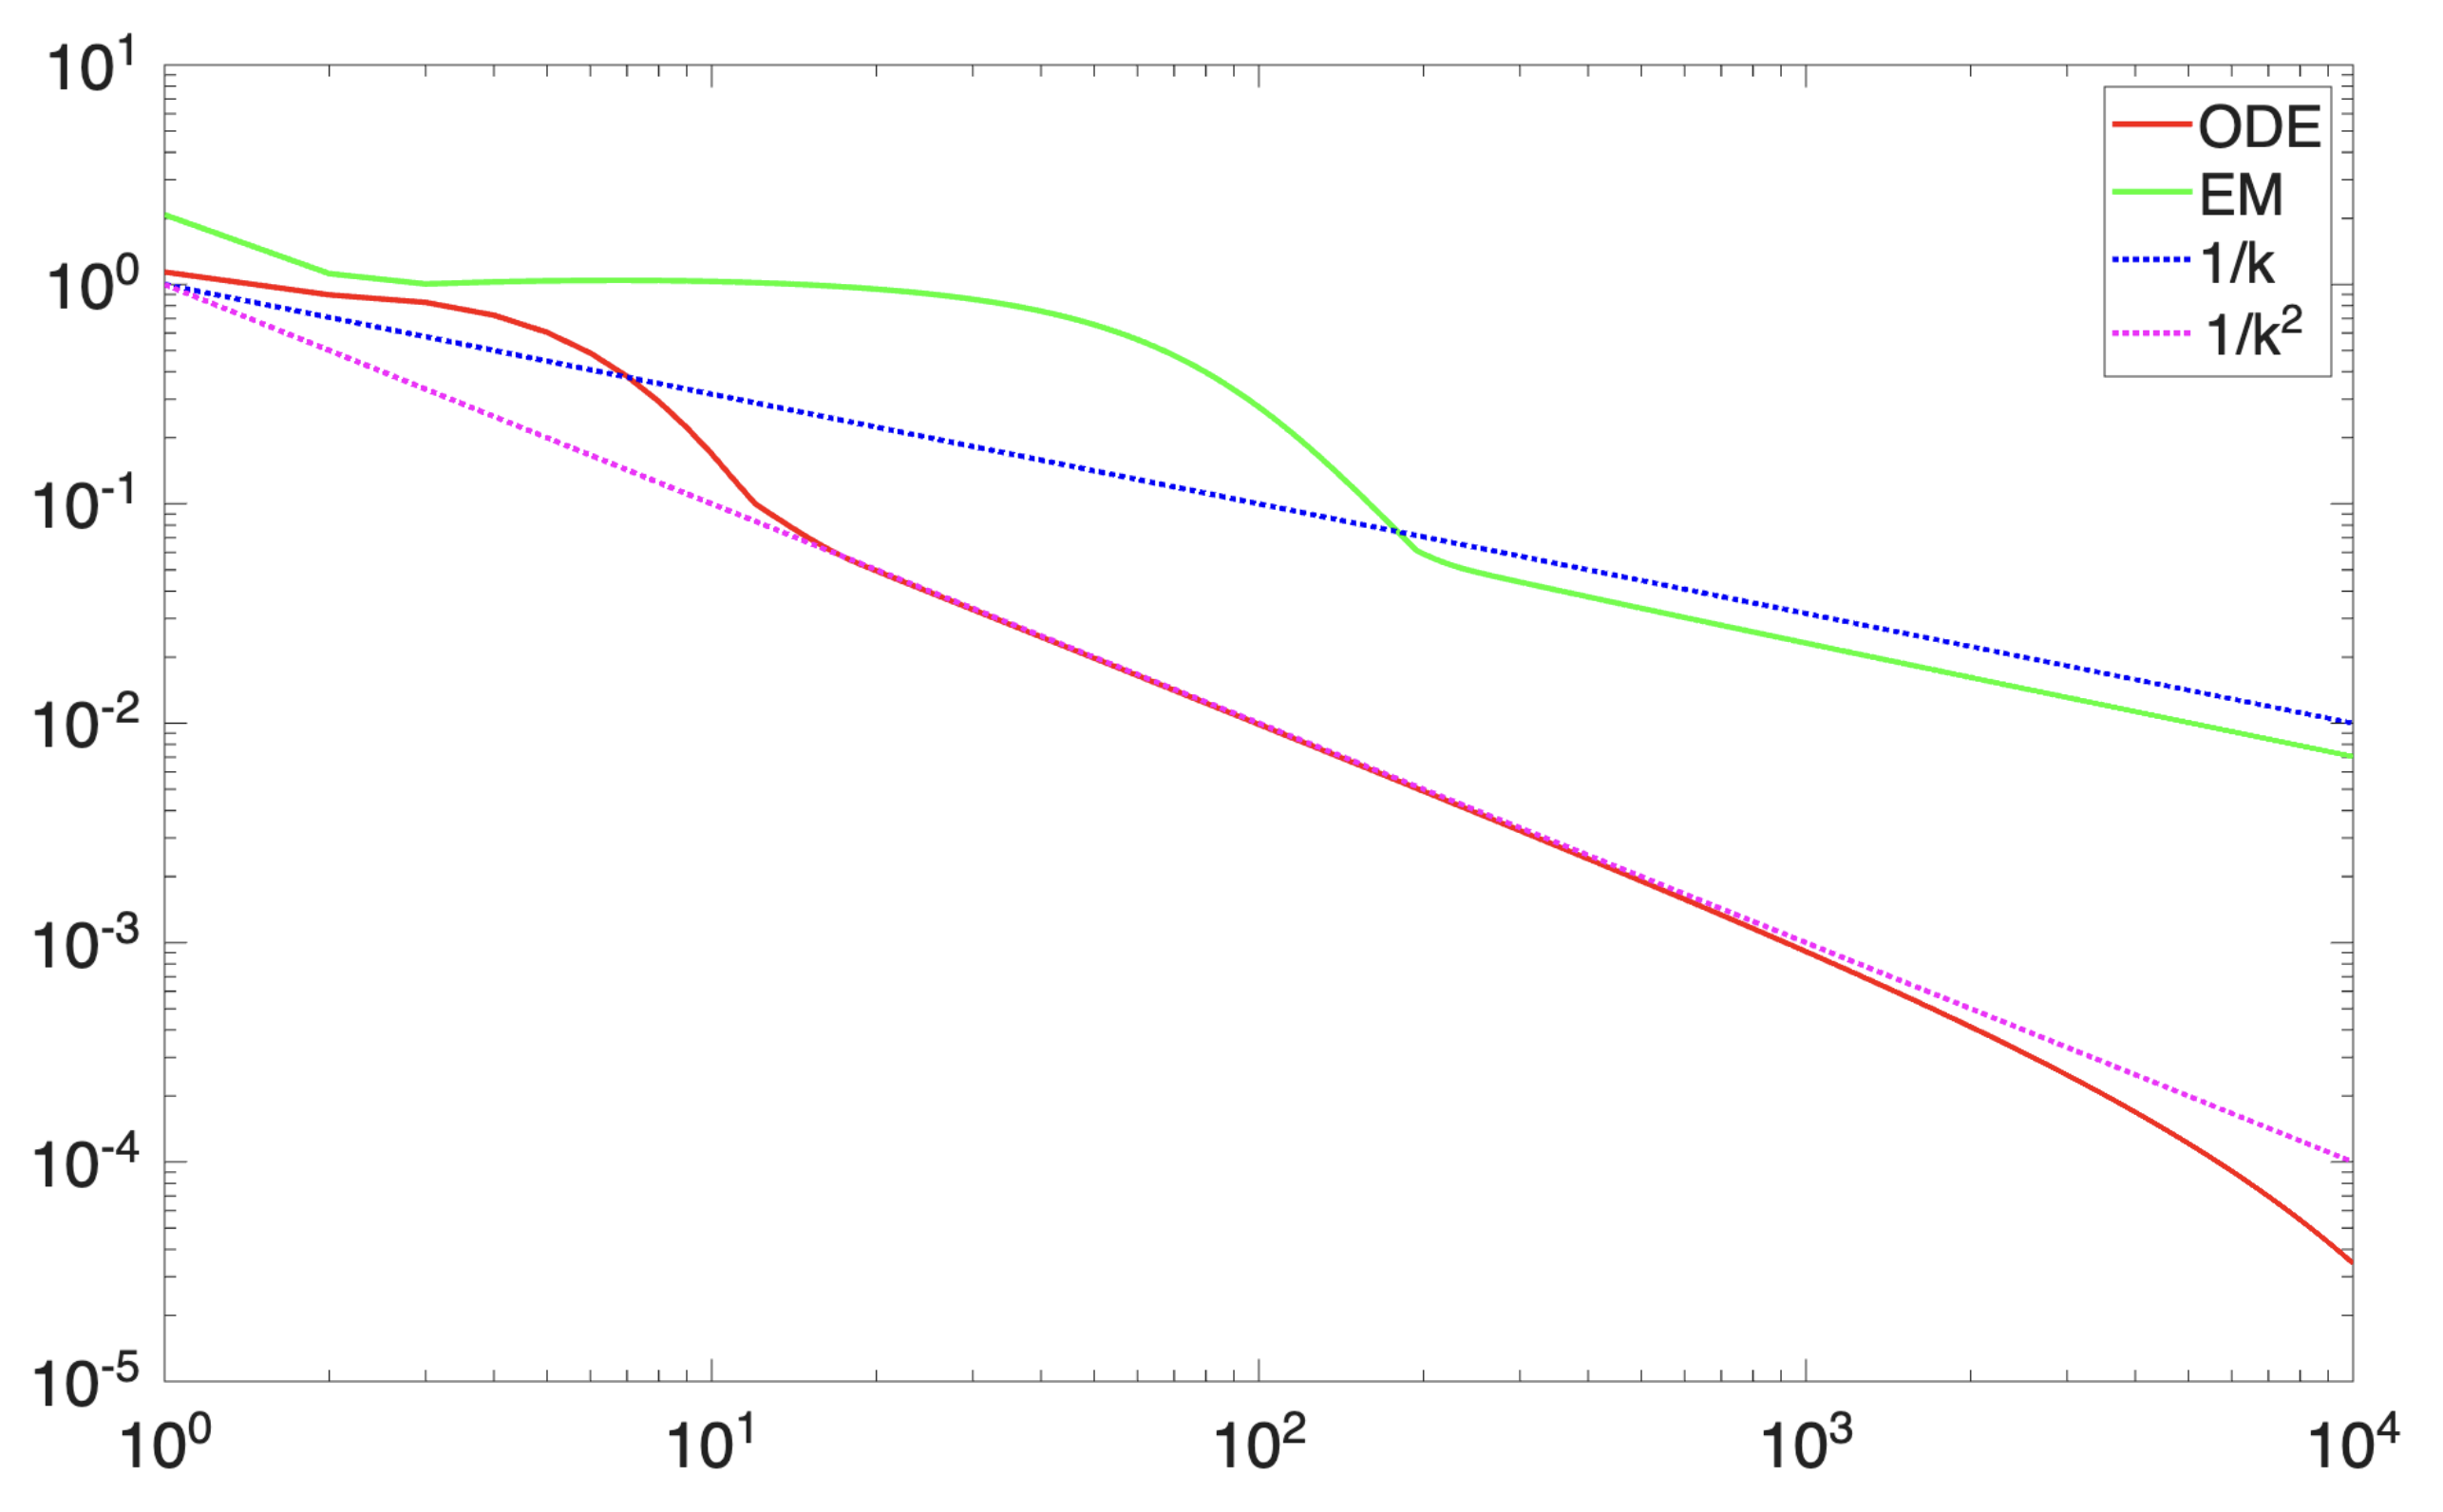
\includegraphics[scale=0.24]{empirical_contraction_rate.png}
	\caption{Empirical results on contraction. y-axis is $\|\Sigma - \Sigma_k\|$ and x-axis is iterations $k$.}
\end{figure*}

\begin{remark}[Acceleration interpretation]
The EM algorithm has a mirror descent structure, which gives a non-asymptotic rate of $O(1/k)$. By analogy with acceleration in convex optimization (Nesterov), the ODE scheme appears to achieve $O(1/k^2)$. This is observed empirically in the paper's Figure~2, but a theoretical proof of this non-asymptotic rate remains an open question.
\end{remark}

Apart from this derivation, they show contraction in Wasserstein and KL (for Lipschitz drift \& score fields).


%% ============================================================
\section{Open Questions}
%% ============================================================

\subsection{Theory}
\begin{itemize}
	\item \textbf{Approximate drift/score and time-discretization:} The current analysis assumes exact drift/score at continuous time. How do discretization errors and neural network approximation errors interact?
	\item \textbf{Non-asymptotic rates:} The Gaussian example empirically suggests $O(1/k^2)$ convergence for the ODE. Can this be proven? What is the structure that enables acceleration?
	\item \textbf{Beyond linear interpolants:} Non-linear interpolants could improve the Lipschitz constant $L_\epsilon$ and tighten the convergence. What is the optimal interpolant design?
	\item \textbf{Condition number dependence:} How does performance scale with the condition number $\chi$ of the forward model?
\end{itemize}

\subsection{Methods}
\begin{itemize}
	\item Extension to \textbf{discrete flow matching} (discrete state spaces).
	\item Extension over \textbf{function spaces}: let $\mathcal F$ be an operator (e.g., PDE solution map) rather than a pointwise function.
\end{itemize}

\subsection{Applications}
\begin{itemize}
	\item What happens under \textbf{model misspecification} of $\mathcal F$?
	\item The method assumes $\mathcal F$ is cheap to query. Can it work when $\mathcal F$ is expensive (e.g., PDE solves)?
	\item Connections to \textbf{simulation-based inference}.
\end{itemize}


\end{document}